\documentclass{article}
\usepackage{graphicx}
\title{Introduction to Wireless Networks Final Review}
\begin{document}
\section{Multiplexing}
We want to allow multiple users to access the same channel. We usually split the
available spectrum. We also have the frequency and time domains to be wary of. 

\textit{frequency domain}: The frequency domain refers to the measuring of a 
mathematical function with respect to its frequency rather than with respect to time.

\textit{time domain}: measuring of functions with respect to time, rather than frequency. 

When we have mutliple users that want to share a channel, we need to think of some way to 
split that channel, this is called \textbf{multiplexing}.

There are usually two major ways of splitting the channel, frequency division and time division.

With frequency division, we assign each comepting signal a special frequency to transmit.

With time division, we split a \textit{frame} into multiple \textit{slots}, which can then be 
occupied by the signals that wish to transmit instructions. Both the uplink and downlink channels
will employ this. However, from the diagram in the ppt, it seems that the slot link in the 
uplink will occupy the nth slot in the downlink. The ith packet in the uplink will occupy the 
n-ith slot in the downlink.

\subsection{Code Division Multiple Access}
With this scheme, we can  use a ``spread spectrum" technique to generate a code for each individual
sender. We break each bit according to a code (usually with bitwise XOR) to generate a code. Then,
we can simultaneously send data for multiple users at once. 

This introduces the \textbf{Near-Far problem}, which denotes the phenomenon where a signal that is
closer to the receiver will be heard stronger and even potentially block one that is farther away. There
are a couple kinds of interference in CDMA, such as \textit{adjacent channel interference}.

\subsection{Narrowband systems}
There are a large number of narrowband systems, such as:
\begin{enumerate}
		\item{\textbf{FDD}}
		\item{\textbf{Narrrowband TDMA and Narrowband FDMA}}
		\item{\textbf{FDMA\ FDD}}
		\item{\textbf{FDMA\ TDD}}
		\item{\textbf{TDMA\ TDD}}
\end{enumerate}

\subsection{Frequency Division Duplexing}
For FDD, we have two different bands, the forward and reverse band. We need a duplexer here to The 
frequency separating the reverse and forward channel is always constant.
\subsection{Time division Multiplexing}
Using this scheme, we use time for forward and reverse link. Then multiple users can share a single
radio channel. There is a different reverse and forward time slot.

\subsection{wideband Systems}
In this scheme there are a large nubmer of transmitters on one channel. 
\subsection{Frequency Dvision Multiplexing Access}
In this scheme, there is one circuit per channel. Because there is only one circuit (circuit switching)
per channel, if the channel is not in use, then it will not be as efficient(similar to circuit switching
in networks). With this scheme, one is continuously and simultaneously transmitting with other senders.
This is usually implemented in narrowband systems.

Compared to TDMA, FDMA uses fewer bits for synchronization and framing, however it also has a higher 
cost for duplexers which are used in base station and subscriber units(duplexers allow for two-way
transmission). This scheme also requires RF filtering to minimize adjacent channel interference.

\textbf{Adjacent Channel Interference} refers to a problem where excess power from an adjacent channel.
So a signal in a given frequency can sometimes feel the effect of a signal in the neighboring 
frequency range. This sometimes happens when the power modulation and regulation is not constant, or 
there is poor frequency control in the system.

Some nonlinear effects of FDMA include:
\begin{enumerate}
		\item{many channels use the same antenna}
		\item{we need to operate at saturation for maximum power efficiency}
		\item{power amplifiers are nonlinear near saturation power}
		\item{nonlinearities cause signal spreading}
		\item{intermodulation frequencies}
		\item{IM are undesired harmonics}: remember harmonics are waves with frequencies that are multiples
				of a given wave.
		\item{interference with other channels in frequency}
\end{enumerate}
\subsection{Time Division Multiple Access}
Here, we have multiple \textit{time slots}, which add together to make a single \textit{frame}. A time slot 
contains only one user, and we can divide a frame so that multiple users send information in their given 
time slot.

We use what's called the \textit{Buffer and Burst } method, which places a buffer where our data is stored.
Becuase of this, the transmission is not continuous, but may occur in short ``bursts" (:)). We can use
digital modulation to send digital data. \textit{Digital Modulation} refers to changing the digital signal
which is outgoing to an analog signal, which is what is used for transmission.

The frame of a single frame consists of several parts: a preamble, information message(where slots come in), and
Trail Bits(to indicate where transmission ends?).

TDMA has these features:
\begin{enumerate}
		\item{single carrier frequency for several users}
		\item{transmission in bursts}: while using buffer and burst method.
		\item{low battery consumption}
		\item{handoff process much simpler than for CDMA}
\end{enumerate}
The efficiency of TDMA depends on the percent of data that contains information.
\subsection{Space Division Multiple Access}
Space Division Multiple Access entails radiating the controls offered by the spot beam antenna. The base 
station can track the user's movements.

It can cover areas with the same frequency as TDMA or CDMA. We use ``sectorized antennas", where spot beam
antennas offer coverage only in a sector of the curcular radius of the antennas. Here, each antenna
can cover only a specified range within the circular radius.  In the future, possibilities include 
dynamically tracking the areas where there are more users, thus improving coverage. 

\subsection{Reverse link problems}
\textbf{reverse link}: the propagation path from user to base station.

The user may use a different propagation path to reach a base station. We have to be careful with this
because mobile batteries limit the amount of possible overhead. We can apply filters to each user to react
differently.

What do SDMA systems do to fix this? We can use adaptive antennas to mitigate these problems. Adaptive antennas 
are useful when we want to account for an increasing user base with ever increasing data requests. These sytems
will allow for better \textit{spectral efficiency}, which will allow us to increase the amount of data for each user.
An adaptive antenna system consists oF multiple antenna elements.
This can help curb interference from physical obstacles, which remains one of the biggest obstacles in wireless network
communication.

This can also help with the case of infinitesimal bandwidth and infinitely fast track ability, creating a unique channel that is free f
rom interference. Then all users communicate at the same time using the same channel.

However, for a perfectly adaptive antenna, one with infinite size would be needed, so a compromise is required. The 
\textbf{INTELSAT IVA} satelite uses a dual beam antenna. This antenna can simultaneously acces two different areas of 
the earth. To increase coverage on two simultaneous hemispheres.
\subsection{Capacity of cellular networks}
\textbf{channel capacity}: The maximum amount of users in a fixed frequency band.
\textbf{radio capacity}: value for spectrum efficiency. 
\section{Medium Access Control in Wireless LANs}
Why do we need Medium Access Controls? The medium is shared(frequency, time,etc...), so we neeed a way of 
determining who is allowed to send information at any given time. If they all sent at  the same time, there
would be collisions and interference. 

What do we want in a MAC? We want to avoid interference among simultaneous transmissions. Also, we would like 
for the entire thing to be distributed, not coordinated by some centralized coordinator.

However, we only guarantee one-hop reliability, that is, how to send the information to the next node, we don't 
concern with how to get it to the final destination. We also want to maximize use of available bandwidth, and fair
allocation of that bandwidth to contending nodes; minimizing delay in sending/receiving messages; and to minimize the
energt consumption of sending/receiving messsages.

Some challenges include:
\begin{enumerate}
		\item{error prone channel}
		\item{limited bandwidth}
		\item{limited communication range}
		\item{limited energy}
		\item{Node mobility}
		\item{Lack of central coordination and lack fo tight time schedule}
\end{enumerate}

We classify different MAC protocols into either \textit{Contention Free } protocols  or \textit{Contention Based}
protocols.

\textbf{Contention-free} protocols try to divide the wireless channel into logical ones that minimize interference.
Usually more applicable to ones with more centralized control. These include TDMA, FDMA ,and CDMA.
\subsection{Contention-based Multiple Access}
For contention-free protocols we can list: \textit{ALOHA} and \textit{Slotted ALOHA}, \textit{CSMA}, \textit{MACA},
and \textit{MACAW}.
\subsection{ALOHA, slotted ALOHA}
for pure (unslotted aloha), the nodes will send information whenever they have information to send. Then, if there
is no ACK in a certain amount of time, we retransmit after a certain amount of time.

For slotted ALOHA, we divide the time into equal time slots and send a certain packet of information at the 
\textit{beginning} of the slot. If the transmission fails, we resend it in a  future slot with a certain probability.
\subsection{CSMA(Carrier Sense Multiple Access)}
The sender first ``senses" the wireless channel, and if it is idle, it starts transmitting. Otherwise if the channel
is in use, the sender will restrain itself from sending information(Don't interrupt). This approach is 
\textit{CSMA with carrier sensing}.

However, we can also define it so that if it detects the channel is busy with a transmission, it will wait a random
amount of time before attempting to send the packet again. The possibility of collisions will go down if this is 
implemented.\textit{CSMA with Collision Avoidance}

\textit{backoff time} The backoff time is selected as a random interval of time. We set our backoff timer to this 
interval and then decrease the timer while the channel is sensed to be idle. It is paused when another transmission
is detected and  the transmission starts when the channel has been idle for more than one DIFS. If the medium is busy,
the transmission is deferred until the end of the current transmission.
\subsection{IEEE 802.11}
The infrastructure for the famous 802.11 protocol is composed of:
\begin{enumerate}
		\item{station(STA)}: terminal with access mechanisms to wireless channel and radio contact to the access
				point.
		\item{Basic Service Set(BSS)}: group of stations using the same frequency.
		\item{Access Point}: station integrated into wireless LAN and distribution system.
		\item{portal}: bridge to other (wired) networks.
		\item{Distribution system}: interconnection network to or from one logical network.
\end{enumerate}
 This protocol is the standard MAC and physical protocol for wireless LANs.

 The MAC layer offers two types of services: distributed coordination function(DCF) and Point Coordination Function.
The \textit{DCF} conbines the physical and virtual sensing.

The way the protocol works is defined below:

\hfill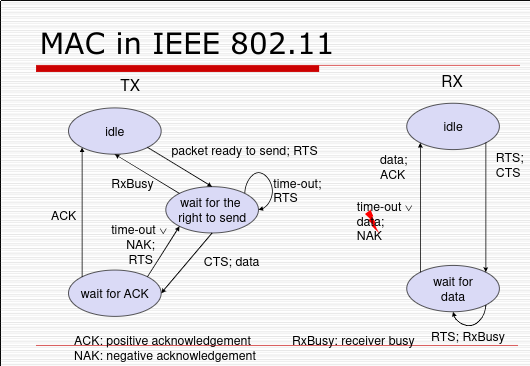
\includegraphics[scale=.50]{wifi}\hspace*{\fill}

The priorities when we want to send packages are determined by different inter frame spaces. Shorter lengths 
indicate higher priority
\begin{enumerate}
	\item{Short Inter Frame Spacing(SIFS)}:  Since they usually need to be sent the fastest (ACK, CTS,polling), these
	packets 
	\item{PIFS}: medium priority, used for time-bounded services.
	\item{DIFS}: lowest priority, for asynchronous data service(not required to be the fastest).
\end{enumerate}
The Point Coordination Function(PCF) is run by the Access Point and coordinates the transmission to its neighbors. There is
the Access Point(AP), which coordinated the transmission of its neighbors. It polls the neighbors one after another,and 
allows them to transmit in round-robin manner. This is not really suitable for multi-hop networks.

Some problems with Carrier sensing include:

\textbf{hidden terminal problem}: When a node can communicate with an AP byt cannot communicate with other networks
communicating with that same AP. The \textbf{exposed terminal problem} refers to when a node cannot send a packet 
to other nodes becuase of \textit{cochannel interference}.The sensing range > receiving range. Also, the 
connection matters only at a receiver's end.

The \textit{near and far terminals}, similar to the ones for other MAC protocols, closer signals can ``drown out" the
signals coming from farther away, even if they are all within range(this is for hidden terminals). 
\textit{Exposed terminals} are ones in which twonodes are transmitting (say A and B), and node C is 
only within range of B. If node C wants to transmit, then it wouldn't
be able to because it would detect the channel, even if it is not necessary. 



\subsection{MACA (Multiple Access Collision Avoidance)}
We don't have the carrier sense, instead we use short signaling packets to get information about the situation. We have 
two types of packets, \textit{RTS}(Request to Send) and \textit{CTS}(Clear to Send). RTS messages are sent to the receiver
with a short packet format. If all is clear, the receiver sends back a CTS packet. These contain only the addresses of the 
two packets and the size of the packets.

This strategy solves the hidden and exposed terminal problems becuase now the sender receives direct confirmation from the 
receiver. Here, no nodes sending to other nodes will give wrong idea about the network situtation.

What are the disadvantages of using this scheme? There are high power consumption issues; the hidden terminal program is
not really solved (RTS packets can still collide); the exposed terminal problem is not really solved either; it only 
provides the ``best effort" service, it doesn't guarantee a packet will be delivered.

 To recap the priority values
\begin{enumerate}
		\item{SIFS(Short IFS)}: for all immediate, high-priority actions(RTS,CTS,ACK,...).
		\item{PIFS(point coordination function IFS)}: used by the centralized controller in PCF scheme when issuing polls.
		\item{DIFS(distributed coordination function IFS)}: used as minimum delay for asynchronous frames contending for
				access.
\end{enumerate}
\textit{SIFS} are the highest priority level.
\textit{PIFS} are used by controller to issue polls. 
\textit{DIFS} are used for everything else (asynchronous).

\section{Wifi}
The wifi standard, since it was started in the 90s, only had support for around two MHz.
The original standard was developed in the 90's, but has continually been increased to allow for greater speeds.
The standard allows for different types of services, such as \textit{distribution service} and \textit{station service}.

When a host in one service set wants to connect to one in another set, it performs ESS-Transition.
\subsection{Distribution Service}
The first distribution service is by \textit{association}. First, a user must connect to an access point.  

The next distribution service is called \textit{disassociation}. With this distribution service, once there is a connection
to the access point, once we want to canel it, we have to send a message to the access point. Then the AP will update its
database. If, for whatever reason, the access point wants to stop offering its service, the AP will just send a signal 
to the connected devices. It's just a notice, doesn't need to wait for a repsonse.

Yet another service is called \textit{reassociation}. When a device connected to an access point wants to reconnect to a 
new one, the base station will send a new reconnect message to the AP and then, if another AP requests the user's info,
the base station can respond with the correct information.

\textbf{ditribution} refers to the service that sends the information obtained from the dissasociation service to the 
correct location. The actual standard doesn't say how to do it, so let's get creative!

\textbf{integration} This service's main function is to allow wired and wireless networks to transfer messages to each
other.

\textbf{Authentication} is the application when we authorize a user according to one of the two methods in the standard:
\begin{enumerate}
		\item{Open System}: Most basic authentication scheme. The base station sends the request for authentication 
				(Authentication Request Frame) to the AP, and it will respond with either a positive or negative 
				response.
\end{enumerate}
Some other services offered by the service:
\textbf{Deauthentication}: When the authentication is going to be cancelled, the base station will also cut connection
with the  Access Point.

\textbf{Privacy}: Becuase originally, any person could have access to a message while it was transmitting, the standard
added the ability to add encryption and decryption when sending the information.

\textbf{Delivery of data}: Just a service that allows the AP and base station to communicate.

When there is a collision detected when the package is sent to the internet(collision), the packet will be returned 
to the place where it originated. Ethernet uses CSMA/CD. Also becuase detecting collision in the internet is usually 
challenging, the standard will use \textit{CSMA/CD}.

The standard alo uses the same queueing options as CSMA/CA(SIFS,...).

The point coordinator will manage the Beacon Frame and let other workstations know that the point coordintor's job. Then,
there will be a contention period. During this period, it changes to dissassociation state until the next point 
coordinator's job begins.

The standard also employs RTS/CTS messages. In the implementation of wifi, there is also the \textit{Hidden Node} problem.
Although using distinct messages to ask for permission to send, these messages themselves can still collide with each other.

\textbf{Frequency Hopping Spread Spectrum} is a method of sending radio signals by switching frequency channels. Different
countries have different settings. Although the Frequency hopping spectrum is quite narrow, the speed at which a signal
can switch frequency makes it seem like it is actually utilizing the entire spectrum.

\textbf{Direct Sequence Spread Spectrum} is a technique aimed at reducing overall signal interference. The spreading of this
signal makes the channel overall more noisy though.

Which one should we use then? 
Because DSSS makes the overall frequency band more noisy, then we shouls only use it when the channel is wide.
\section{Misc.}
\subsection{GSM}
The \textit{Global System for Global Communications} was develeoped in the mid 90s for 2G mobile communications. Originally,
it was meant to be a packet-switched system, later, packet-based functionality was added in support for internet connections.

The  main parts of the GSM infrastructure involve:
\begin{enumerate}
		\item{Base Station Subsystem}: base station and their controllers
		\item{Network and Switching Subsystem}:``core network".
		\item{GPRS}: optional part which allows internet packet-based connections.

				
\end{enumerate}
\subsection{Base Station Subsystem} 
Cell phones will search for the nearest substation when trying to connect. There are different types of statios which allow
for different distances to be searched.
\section{The Wi-Fi standard}
The wifi standard operates on WLANs and manages to work efficiently with the sister network Ethernet.
\end{document}
